\documentclass[12pt, a4paper]{article}

\usepackage{array}
\usepackage[portuguese]{babel}
\usepackage{chngpage}
\usepackage{float}
\usepackage[a4paper, margin=2cm]{geometry}
\usepackage{graphicx}
\usepackage{hyperref}
\usepackage{setspace}
\usepackage{xcolor}

\title{\Huge \textbf{Computação Gráfica \\ \Large Trabalho Prático -- Fase I}}
\date{2 de março 2025}
\author{Grupo \textbf{\color{red} TODO}}

\begin{document}

\begin{center}
    
\includegraphics[width=0.25\textwidth]{res/cover/EE-C.eps}
\end{center}

\chardef\_=`_
\onehalfspacing
\setlength{\parskip}{\baselineskip}
\setlength{\parindent}{0pt}
\def\arraystretch{1.5}

{\let\newpage\relax\maketitle}
\maketitle
\thispagestyle{empty}

\vspace*{\fill}

\begin{adjustwidth}{-2cm}{-2cm} % These values only need to be large enough to center the table
    \begin{center}
        \begin{tabular}{>{\centering}p{0.25\textwidth}
                        >{\centering}p{0.25\textwidth}
                        >{\centering}p{0.25\textwidth}
                        >{\centering\arraybackslash}p{0.25\textwidth}}
            
\includegraphics[width=3.5cm]{res/cover/A104437.png} &
            
\includegraphics[width=3.5cm]{res/cover/A104348.png} &
            
\includegraphics[width=3.5cm]{res/cover/A90817.png} &
            
\includegraphics[width=3.5cm]{res/cover/A104179.png} \\

            Ana Oliveira & Humberto Gomes & Mariana Cristino & Sara Lopes \\
            A104437      & A104348        & A90817           & A104179
        \end{tabular}
    \end{center}
\end{adjustwidth}

\pagebreak

\begin{abstract}
    \textbf{\color{red} TODO - resumo}
\end{abstract}

\section{\emph{Generator}}

\subsection{Gerador de primitivas gráficas}
O generator é responsável por gerar primitivas gráficas criando ficheiros com os
vértices e faces triângulares dessas mesmas primitivas.

Para gerar primitivas gráficas, o generator recebe um argumento com o nome
da primitiva que iremos gerar, mais argumentos como altura, raio, slices e stacks,
dependendo da primitiva, e por fim recebe ainda um último argumento com o caminho relativo
do ficheiro que iremos criar.
\subsection{Figuras}
Neste fase o generator deve conseguir gerar as seguintes figuras: um plano, um cubo,
uma esfera e um cone. Como extra, também desenvolvemos a geração do cilíndro e do torus.

A forma como o utilizador deve executar o generator é descrita na mensagem de erro, quando
o utilizador não utiliza o generator corretamente:
\begin{verbatim}
Wrong usage. Here's the correct one:
./generator plane    <length>      <divisions>                     <file>
./generator box      <length>      <grid>                          <file>
./generator sphere   <radius>      <slices>      <stacks>          <file>
./generator cone     <radius>      <height>      <slices> <stacks> <file>
./generator cylinder <radius>      <height>      <slices> <stacks> <file>
./generator torus    <majorRadius> <minorRadius> <slices> <stacks> <file>
\end{verbatim}
Devemos primeiro ir para a diretoria build e depois executar o generator, como descrito em cima.

No generator vemos se o número de argumentos é válido conforme a figura e vemos se alguns valores
inseridos são inteiros ou doubles e se são números positivos. Se algo for inválido é nos mostrada
a mensagem de erro apresentada anteriormente.

\subsection{Ficheiro}
Depois de gerarmos a figura, vamos guardar a informação no ficheiro pedido.

Para o formato dos ficheiros gerados, decidimos seguir o formato Wavefront OBJ (OBJ ou .OBJ),
um formato de ficheiro usado para representar geometria 3D, muito usado na indústria 3D.
Este formato tem a vantagem de, para definir faces, não termos de repetir as coordenadas dos
vértices, apenas temos de indicar o índice dos vértices dessa face, o que diminui o tamanho do
ficheiro.

Neste formato, para definir um vértice colocamos 'v' seguido das coordenadas do vértice.
Por exemplo, para representar a origem, o vértice de coordenadas (0,0,0), fazemos:
\begin{verbatim}
v 0 0 0
\end{verbatim}
Para definir uma face triângular colocamos 'f' seguido dos 3 índices dos vértices dessa face.
Por exemplo, para representar uma face triângular, formada pelo primeiro, segundo e terceiro
vértice do ficheiro, fazemos:
\begin{verbatim}
f 1 2 3
\end{verbatim}

\subsection{Cone}
Para gerar um cone temos de indicar o raio da base do cone (radius), a altura do
cone (height), o número de slices, o número de stacks e o caminho relativo para o
ficheiro que iremos criar com os vértices e faces triangulares do cone (file).

Para calcular os vértices e as faces triangulares de um cone, primeiro tivemos
de tomar uma decisão. No enunciado apenas diz que a base do cone deve estar no
plano XZ. Assim, sabemos que a ordenada (y) do centro da base do cone é nula
mas nada nos é dito sobre a abscissa (x) e sobre a cota (z) do centro da base
do cone. Para o cone estar consistente com as restantes figuras e para facilitar
os cálculos, decidimos que a base do cone estaria centrada na origem, ou seja,
teria abcissa e cota nulas.

Depois, começamos por calcular os vértices do cone.

O primeiro vértice é a origem e o último vértice tem abscissa e cota nulas e
tem ordenada igual à altura do cone.
$$
P_0 = (0, 0, 0)
\hspace{1cm}
P_n = (0, height, 0)
$$

\begin{figure}[H]
    \centering
    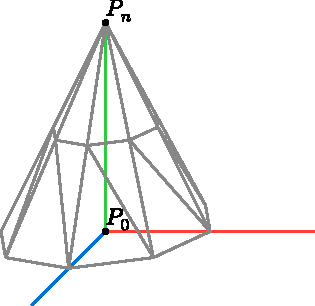
\includegraphics[width=0.4\textwidth]{res/figures/Cone1.pdf}
    \caption{
        Cone gerado, o seu primeiro vértice ($P_0$) e o seu último vértice ($P_n$).
    }
\end{figure}

Também calculamos os restantes vértices. Para cada stack, calculamos X
vértices, sendo X o número de slices.

\begin{figure}[H]
    \centering
    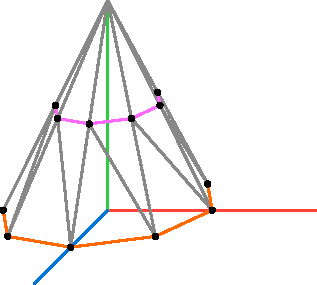
\includegraphics[width=0.4\textwidth]{res/figures/Cone2.pdf}
    \caption{
        Cone com 2 stacks e os vértices (visíveis) calculados em cada stack.
    }
\end{figure}

Como podemos ver pela imagem os vértices calculados para uma stack,
teem todos a mesma ordenada. Podemos obter a ordenada da seguinte forma,
considerando que começamos pela iteração 0:
$$
y = (height/stacks) * iteracao
$$
Para cada stack, ainda obtemos o raio da circunferência formada pelos vértices dessa stack,
que será usado posteriormente para calcular abcissas e cotas.
Para obter o raio, utilizamos a regra de semelhança de triangulos que nos diz que triangulos
semelhantes teem o comprimento dos lados proporcionais:
$$
new_radius = ((height - y) * radius) / height
$$
Depois, ainda numa stack, por cada slice vamos calcular então um vértice.
Depois de termos os vértices, falta calcular as faces triangulares. Primeiro vamos calcular
as faces da base do cone, depois vamos calcular as faces laterais do cone e por fim iremos
calcular
\section{\emph{Engine}}

\textbf{\color{red} TODO - \emph{engine}}

\section{Resultados obtidos}

\textbf{\color{red} TODO - resultados}

\section{Conclusão e Trabalho Futuro}

\textbf{\color{red} TODO - conclusão}

\begingroup
\section{Bibliografia}
\renewcommand{\section}[2]{}

\begin{thebibliography}{9}
    \bibitem{exemplo}
        \href{https://youtu.be/dQw4w9WgXcQ}{Um item de exemplo na bibliografia}
\end{thebibliography}
\endgroup

\end{document}
